\section{Implementation}
\label{sec:impl}

%\begin{spacing}{0.9}
We implement \name in Linux v4.9 and TensorFlow v1.14. We change the Linux kernel for memory profiling; We change the TensorFlow runtime system for page migration. The statistics of kernel modification given by \textit{git diff} is 17 files changed, 587 insertions(+), 18 deletions(-); The statistic of TensorFlow modification given by \textit{git diff} is 33 files changed, 2425 insertions(+), 37 deletions(-).

\name introduces three APIs to trigger/stop memory profiling and identify DNN layers, which are \texttt{start\_profile()}, \texttt{end\_profile}(), and \texttt{add\_layer()}. \texttt{start\_profile()} triggers a system call to enable tracking main memory accesses, and enables tracking of memory allocation/deallocation to record lifetime information of data objects. \texttt{add\_layer()}, placed at the end of each layer, informs the runtime system of where is each layer to determine migration interval. Adding \texttt{start\_profile()} and \texttt{end\_profile()} includes only two lines of changes to the DNN model. Adding \texttt{add\_layer()} includes \~10-100 lines, depending on how many layers there are in the DNN model. Adding those APIs do not impact execution correctness of DNN training. 
%\end{spacing}


%\textcolor{green}{ \name expects three user annotations to trigger profile and page migration for DNN models. These annotation are implemented as TenorFlow operations and provided Python interface. And all of the annotations do not effect the computation of DNN models \texttt{start\_sentinel\_profile()} and \texttt{end\_sentinel\_profile()} specify the profiling step. Those APIs trigger system call to track main memory page access. Meanwhile those APIs enables tracking TensorFlow default allocater/deallocator to record tensor lifetime information.  Annotation \texttt{sentinel()} marks the minimum migration granularity of \name. \name expects user to place this annotation at the end of each DNN layer. Note that \name guarantees execution correctness regardless of where annotations are placed. }


\begin{figure}
\centering
%\vspace{-20pt}
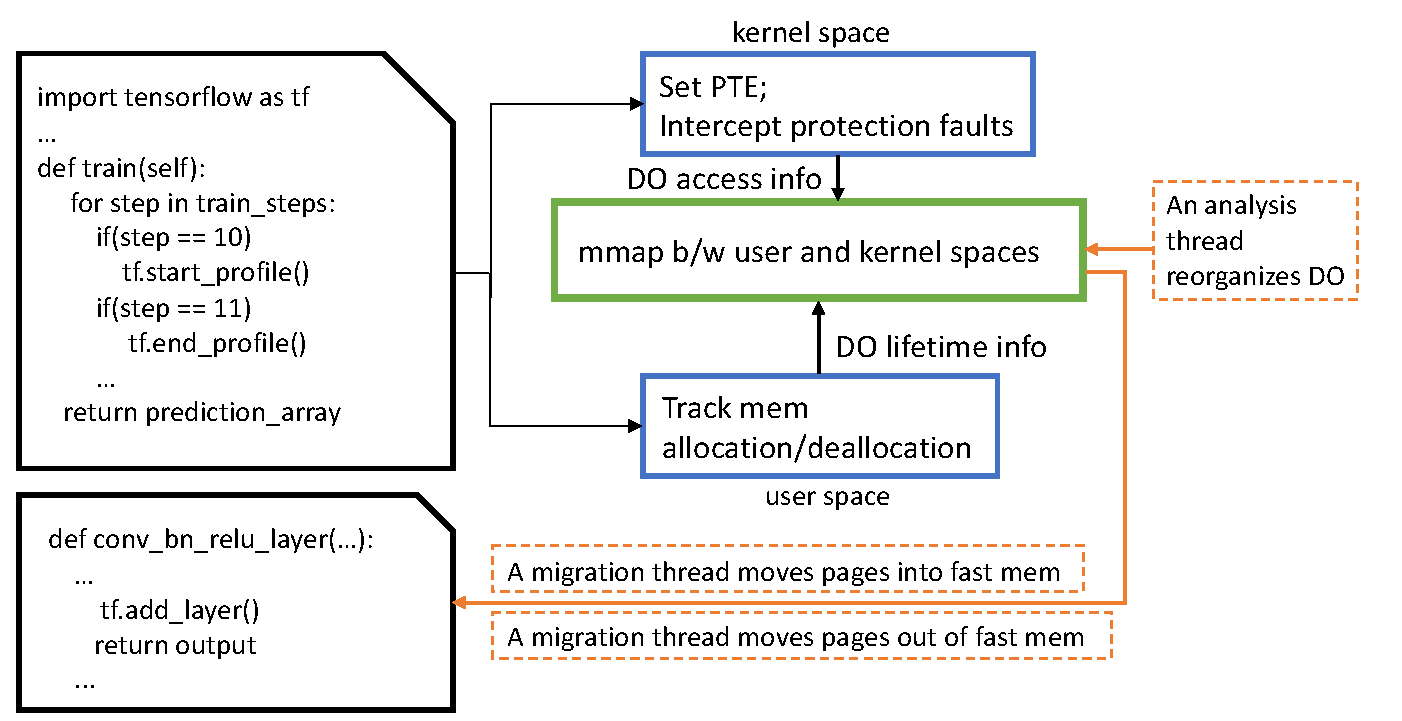
\includegraphics[width=0.48\textwidth]{figures/impl.pdf}
\vspace{-20pt}
\caption{Overview of \name implementation. ``DO'' in the figure stands for ``data objects''.}
\vspace{-15pt}
\label{fig:impl}
\end{figure}

%\textcolor{red}{Add a figure to explain the impl. The figure includes the user annotation, the helper threads for data migration, and the runtime thread to analyze profiling results and re-organize data.}

%\textcolor{green}{ \name implemenation includes kernel modification and TensorFlow Runtime modification.
%}

%\begin{spacing}{0.9}
Figure~\ref{fig:impl} shows some implementation details. \textcolor{check}{During the profiling step, \name collects memory access information from OS; \name also collects lifetime information for each tensor from the TensorFlow runtime. After the profiling step,}  \name uses three helper threads: one for information analysis to determine migration interval and making migration decision, one for data migration from fast to slow memory, and one for the migration in the opposite way. The two migration threads work in parallel to accelerate migration. \name uses the Linux system call \texttt{move\_pages()} to migrate pages. \textcolor{check}{
\name extends TensorFlow memory allocation and free functions (i.e., \textit{AlignedMalloc()} and \textit{AlignedFree()}) by adding our customized data reorganization policy. Before the iterative training happens, tensor are allocated in slow memory. After collecting the profiling results, \name manages data allocation and migration.}
%\end{spacing}

%\textcolor{jie}{\name replaces TensorFlow posix allocation and free interfaces(i.e., \textit{AlignedMalloc()} and \textit{AlignedFree()}) with customized memory managements APIs. Specifically, \name preallocates a fixed size of fast memory. All the data objects in DNN training placed in slow memory initially. After getting the profiling result, \name allocates short-lived data objects in reserved fast memory space. The size of reserved space is determined by profiling result. Short-lived data objects will be allocated in slow memory if the reserved fast memory size is not enough. Short-lived data objects never migrate in HM. }

%\textcolor{green}{Figure~\ref{fig:impl} shows \name implementation details. \name gets data object access information from OS and data object lifetime information from TensorFlow Runtime. \name manages kernel mmap space for user and kernel space communication. \name allocates each data object in at least on page to obtain data object access information during the profiling. After the profiling, \name leverages a analysis thread to handle false sharing data objects and reorganize data objects allocated during the profiling step. Meanwhile \name uses two threads for page migration between fast memory and slow memory.}